\chapter{Hardwaredesign}
\section*{Version}
\begin{table}[h]
	\centering
	\begin{tabularx}{\textwidth - 2cm}{|l|l|l|X|}
	\hline
	Dato			& Version			& Initialer 		& Ændring										\\ \hline
	01. november 			& 1 				& Alle				& Første udkast. 						\\ \hline
	09. december 			& 2 				& LS				& Tilføjet tachometer.					\\ \hline
	10. december 			& 3 				& KE				& Tilføjet distancesensor.				\\ \hline

	\end{tabularx}
\end{table}
\clearpage

\section{Strømforsyning}
\subsection{Printudlæg}

For at implementere kredsløbet i figur \ref{fig:bil_psu} på side \pageref{fig:bil_psu} er der udarbejdet et PCB layout for strømforsyningen.
Dette kan ses i figur \ref{fig:bil_psu_pcb}. 
Under udlægget af printet er der taget forbehold for at minimere arealet af strømsløjfer, som ligger i forbindelse med den skiftende udgang samt returveje derfra på LM26003. Ydermere er der også forsøgt at give så god elektrisk kontakt som muligt ved hjælp af brede printbaner til de komponenter, som forventes at trække en stor, evt. skiftende, strøm.
Dette kan ses i området omkring 3V udgangen fx, da diode, spole, udgang samt kondensator ligger helt op ad hinanden. 
De kredse, som ligger i forbindelse med tilbagekoblingen til LM26003 ligger på den 'nedre' del af printet for at minimere støjen fra de skarpe flanker på LM26003's udgang (ben 1-3 og 11-13).
Grundet at skolens komponentlager ikke lå inde med keramiske kondensatorer i størrelsen 6.8 $\mu F$ er der i stedet sat 7 parallelkoblede kondensatorer i på hver 1 $\mu F$.

\vfill

\begin{figure}[h]
\centering
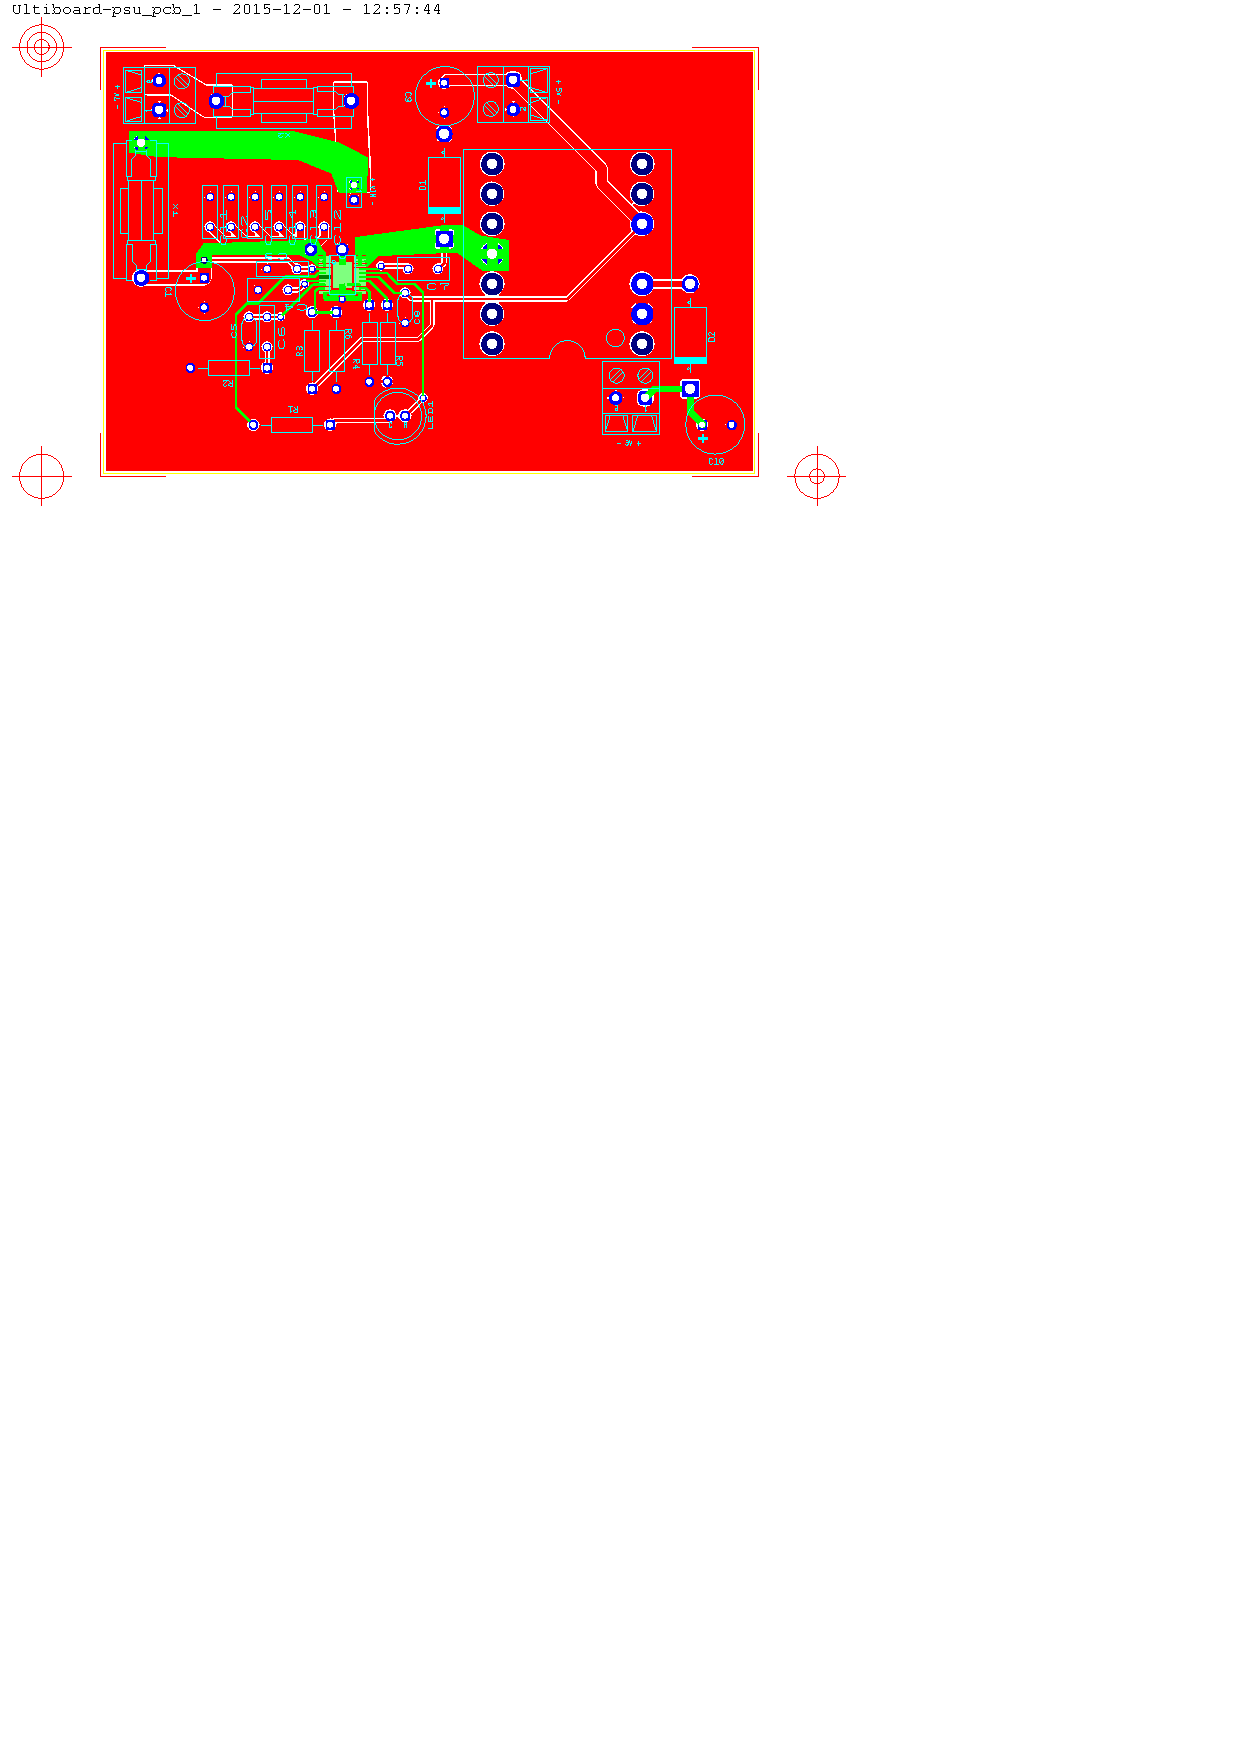
\includegraphics[angle=90,height=\textheight-9cm, clip=true, trim=50 615 234 25]{../fig/diagrammer/bil/psu_pcb_twoside}
\caption{Bilens strømforsyning på PCB}
\label{fig:bil_psu_pcb}
\end{figure}

\clearpage

\subsection{Test}

For at teste strømforsyningen er denne koblet op mod en laboratoriespændingsforsyning indstillet til 7.2V DC.
\section{H-bro - Motorstyring} \label{sec:hwi_motor_driver}
\subsection*{Ultiboard}

Efter at have designet motorstyrings kredsløbet fra figur \ref{fig:MultiSim_HBro} på side \pageref{fig:MultiSim_HBro} i MultiSim bliver det overført til Ultiboard. Her er printet lagt ud med henblik på at reducerer EMC støj fra printet. Printet er delt op i 2 dele. Et med signaler fra PI på 3,3 V ydeste til højre på figur \ref{fig:Ultiboard_Print_H_Bro}. Et til 5V til det logiske kreds på L298N og 7,2V til motor forsyning. De 2 sidste er så vidt muligt holdt væk fra signaler fra PIen. De baner til 7,2V motor forsyning til og fra L298N er gjort så korte som muligt og tæt på returbaner. Så der undgås store strømloops der kan lave en masse EMC støj. Der er desuden lavet et ground plane der også er med til at reducere EMC støj.

\begin{figure}[h]
	\centering
	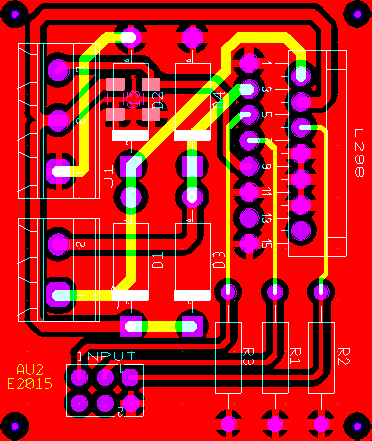
\includegraphics[width=\textwidth* 4/10, angle =90]{../fig/billeder/Ultiboard_H_Bro}
	\label{fig:Ultiboard_H_Bro}
	\caption{Ultiboard H-Bro}
\end{figure}

\begin{figure}[h]
	\centering
	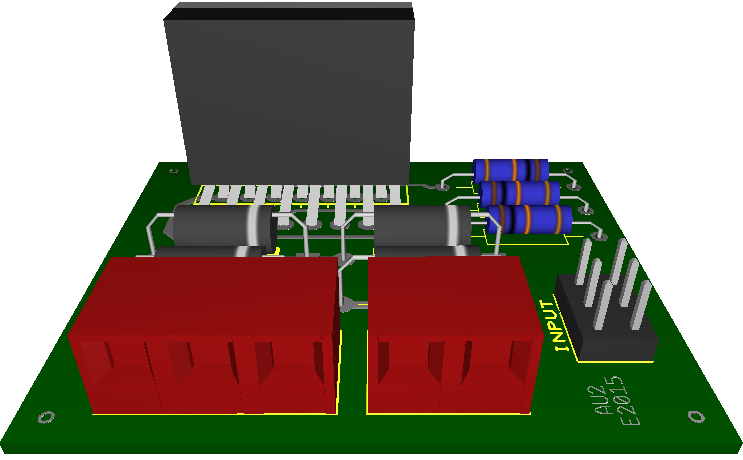
\includegraphics[width=\textwidth* 5/10]{../fig/billeder/Ultiboard_Print_H_Bro}
	\label{fig:Ultiboard_Print_H_Bro}
	\caption{Ultiboard 3D view af print for H-Bro}
\end{figure}

\clearpage
\subsection*{Færdig print}



\begin{figure}[h]
	\centering
	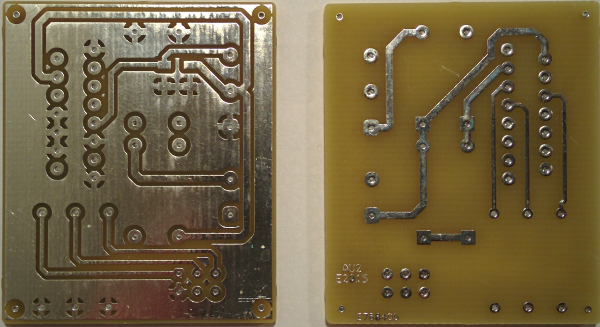
\includegraphics[width=\textwidth* 7/10]{../fig/billeder/Ultiboard_Print_Bare}
	\label{fig:Ultiboard_Print_H_Bro_Bare}
	\caption{Print for H-Bro før komponenter monteret}
\end{figure}

\clearpage
\section{Tachometer} \label{sub:systemarkitektur_tachometer}

For at måle hastigheden af bilen, er det nødvendigt at designe en form for tachometer. Kravene til komponenten er at det skal være kompakt, være strømbesparende og være inden for rimelige grænser prismæssigt. Da DC-motoren som driver bilen er præfabrikeret, og der er gearing før momentet når til hjulene, bliver det hurtigt besværligt at skulle konstruere noget inde ved motoren. Alternativt er der plads ved bilens baghjul, hvilket der vælges at gå frem efter. Gruppen forslog tre muligheder, hvoraf en blev valgt til design/realiseringsfasen.

Her ses de 3 foreslåede muligheder:

\begin{enumerate}
	\item Lys-modtager/sender, som, via en skive med et prædefineret antal huller, kan detektere lys sendt fra senderen ind på skiven og detektere lyset, når det kommer igennem et af hullerne. Derved vil der kunne omregnes fra hvert hul detekteres til en konkret hastighed.
	\item Induktiv føler, som via nogle metalstykker monteret på indersiden af hjulet og en føler skulle detektere en ændring i magnetfelt, når metalstykkerne passerede føleren. På samme måde kunne dette omregnes til en konkret hastighed.
	\item Hall-switch/Reed rør, der fungerer på tilnærmelsesvist samme måde som den induktive føler, men med små magneter monteret på indersiden af hjulet. 
\end{enumerate}

Gruppen valgte at fortsætte med metode 3 - Hall-switch af typen TLE4905L \cite{lib:tacho}. 

En Hall switch kan detektere ændring i magnetfelt og via en schmittrigger trækker den signalet til ground, når der er en magnet tilstede og en høj puls hvis der ikke er. På bilens hjul er fem akser, som er ligeligt fordelt over hjulets omkreds. Ved at montere en magnet på hver af akserne, kan der opnås en stor mængde data, som kan omregnes til en hastighed. 

\begin{figure}[h]
\centering
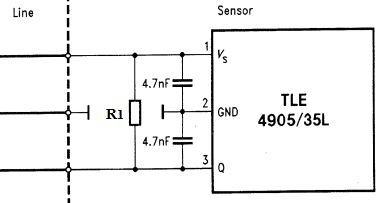
\includegraphics[scale=1]{../fig/billeder/tle4905L_application_circuit.png}
\caption{Anbefalet applikations kredsløb for TLE4905L}
\label{fig:tle4905L_app_circuit}
\end{figure}

På figur \ref{fig:tle4905L_app_circuit} ses det anbefalede applikations kredsløb for hall-switchen. I databladet kan aflæses at forsyningsstrøm ligger mellem 4mA og 8mA, da vi ønsker at trække strømmen fra et batteri, forsøges det at lægge strømmen så lavt som muligt - 4mA. Via ohms lov kan vi udregne R1 til at give ca. $1.2k\Omega$

\begin{equation}
R1 = \dfrac{5V}{4mA} = 1.25\cdot 10^3 \Omega
\end{equation}

Derved kan vi sætte $R1 = 1.25k\Omega \approx 1.2k\Omega$

TLE4905L forventes at blive monteret på bilens højre forhjul, på en måde, så kredsløbet ikke bliver forstyrret for meget af rystelser osv. Som udgangspunkt blev det valgt at implementere tachometeret, således at det kunne aflæses direkte af PI'en, men det viste sig at være særdeles besværligt at komme i kontakt med PI'ens timing og derved kunne udregne hastigheden for bilen. Faktisk viste det sig så besværligt at, der på et relativt tidligt tidspunkt blev indført en PSoC i projektet, som skulle fungere både som en master-slave enhed. Derved kan vi bibeholde \IIC kommunikationen og samtidig have et meget lettere interface, eftersom PSoC'en er lettere at arbejde med, på et mere lavpraktisk niveau end PI'en
% ++++++++++++ Controller PSoC Master klassen ++++++++++++++
\subsubsection{Boundary-klasse: DistanceSensor}

Denne klasse har til formål at styre kommunikation mellem Pi og afstandssensorerne, der er valgt at benytte I2C-kommunikation til dette. De 4 afstandssensorer er navngivet efter deres respektive placering på bilen: ''Front Left'' = ''FL'', ''Front Left'' = ''FL'' ''Front Left'' = ''RL'', ''Rear Right'' = ''RR'', herefter funktion  \texttt{getDistance("name")} kaldes udefra med navnet på den ønskede sensor som parameter, og afstanden returneres i cm. Afstandene gemmes i midlertidige variabler. Desuden skrives der til den globale Log ved klasseinitiering og klassenedlæggelse, samt ved eventuelle forekomster af fejl.

\begin{figure}[h]
\centering
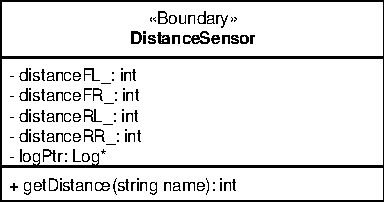
\includegraphics[]{../fig/diagrammer/bil/cd_distancesensor.pdf}
\caption{Klassebeskrivelse af boundary-klassen DistanceSensor}
\label{fig:cd_distancesensor}
\end{figure}

\textbf{Attributter}

\begin{table}[h]
	\begin{tabularx}{\textwidth}{| Z | Z | L{10cm} |} \hline
		Navn & Type & Beskrivelse \\\hline
		\texttt{distanceFL\_} & \texttt{int} 		& Midlertidig variabel der indeholder afstanden fra forreste venstre afstandssensor.\\\hline
		\texttt{distanceFR\_} & \texttt{int} 		& Midlertidig variabel der indeholder afstanden fra forreste højre afstandssensor.	\\\hline
		\texttt{distanceRL\_} & \texttt{int} 		& Midlertidig variabel der indeholder afstanden fra bagerste venstre afstandssensor \\\hline
		\texttt{distanceRR\_} & \texttt{int} 		& Midlertidig variabel der indeholder afstanden fra bagerste højre afstandssensor.	\\\hline
		\texttt{logPtr\_} 	 & \texttt{log*} 		& Pointer til at skrive i den globale Log											\\\hline
	\end{tabularx}
	\caption{Attributter for klassen DistanceSensor}
	\label{table:attr_distancesensor}
\end{table}
\clearpage

\textbf{Metoder}

\begin{table}[h]
	\begin{tabularx}{\textwidth}{| L{2.5 cm} | Z |} \hline
		Prototype 	& \texttt{int getDistance(string name)} \\\hline
		Parametre 	& \texttt{name} \newline Navnet på den sensor som der skal læses fra. Kan rumme én af fire muligheder "FL", "FR", "RL" og "RR". \\\hline
		Returværdi 	& \texttt{int} \newline Seneste afstandsmåling for den pågældende sensor. Værdien er angivet i cm. \\\hline
	\end{tabularx}
	\caption{Metodebeskrivelse for \texttt{getDistance}}
	\label{table:met_getdistance}
\end{table}
\clearpage